\documentclass[8pt]{beamer}

\useoutertheme{infolines}
\usecolortheme[rgb={0.65,0.15,0.25}]{structure}
\beamertemplatenavigationsymbolsempty
%\AtBeginSubsection

% Packages
\usepackage[latin1]{inputenc}
\usepackage{color}
\usepackage{xspace}
\usepackage{dsfont, stmaryrd}
\usepackage{amsmath, amsfonts, amssymb, stmaryrd}
\usepackage{epsfig}
\usepackage{tikz}
\usepackage{url}
\usepackage{/home/robin/LATEX/Biblio/astats}
\usepackage{graphicx}
\usepackage{xspace}

% Maths
% \newtheorem{theorem}{Theorem}
% \newtheorem{definition}{Definition}
\newtheorem{proposition}{Proposition}
% \newtheorem{assumption}{Assumption}
% \newtheorem{algorithm}{Algorithm}
% \newtheorem{lemma}{Lemma}
% \newtheorem{remark}{Remark}
% \newtheorem{exercise}{Exercise}
% \newcommand{\propname}{Prop.}
% \newcommand{\proof}{\noindent{\sl Proof:}\quad}
% \newcommand{\eproof}{$\blacksquare$}

% \setcounter{secnumdepth}{3}
% \setcounter{tocdepth}{3}
\newcommand{\pref}[1]{\ref{#1} p.\pageref{#1}}
\newcommand{\qref}[1]{\eqref{#1} p.\pageref{#1}}

% Colors : http://latexcolor.com/
\definecolor{darkred}{rgb}{0.65,0.15,0.25}
\definecolor{darkgreen}{rgb}{0,0.4,0}
\definecolor{darkred}{rgb}{0.65,0.15,0.25}
\definecolor{amethyst}{rgb}{0.6, 0.4, 0.8}
\definecolor{asparagus}{rgb}{0.53, 0.66, 0.42}
\definecolor{applegreen}{rgb}{0.55, 0.71, 0.0}
\definecolor{awesome}{rgb}{1.0, 0.13, 0.32}
\definecolor{blue-green}{rgb}{0.0, 0.87, 0.87}
\definecolor{red-ggplot}{rgb}{0.52, 0.25, 0.23}
\definecolor{green-ggplot}{rgb}{0.42, 0.58, 0.00}
\definecolor{purple-ggplot}{rgb}{0.34, 0.21, 0.44}
\definecolor{blue-ggplot}{rgb}{0.00, 0.49, 0.51}

% Commands
\newcommand{\backupbegin}{
   \newcounter{finalframe}
   \setcounter{finalframe}{\value{framenumber}}
}
\newcommand{\backupend}{
   \setcounter{framenumber}{\value{finalframe}}
}
\newcommand{\emphase}[1]{\textcolor{darkred}{#1}}
\newcommand{\comment}[1]{\textcolor{gray}{#1}}
\newcommand{\paragraph}[1]{\textcolor{darkred}{#1}}
\newcommand{\refer}[1]{{\small{\textcolor{gray}{{\cite{#1}}}}}}
\newcommand{\Refer}[1]{{\small{\textcolor{gray}{{[#1]}}}}}
\newcommand{\goto}[1]{{\small{\textcolor{blue}{[\#\ref{#1}]}}}}
\renewcommand{\newblock}{}

\newcommand{\tabequation}[1]{{\medskip \centerline{#1} \medskip}}
% \renewcommand{\binom}[2]{{\left(\begin{array}{c} #1 \\ #2 \end{array}\right)}}

% Variables 
\newcommand{\Abf}{{\bf A}}
\newcommand{\Beta}{\text{B}}
\newcommand{\Bcal}{\mathcal{B}}
\newcommand{\Bias}{\xspace\mathbb B}
\newcommand{\Cor}{{\mathbb C}\text{or}}
\newcommand{\Cov}{{\mathbb C}\text{ov}}
\newcommand{\cl}{\text{\it c}\ell}
\newcommand{\Ccal}{\mathcal{C}}
\newcommand{\cst}{\text{cst}}
\newcommand{\Dcal}{\mathcal{D}}
\newcommand{\Ecal}{\mathcal{E}}
\newcommand{\Esp}{\xspace\mathbb E}
\newcommand{\Espt}{\widetilde{\Esp}}
\newcommand{\Covt}{\widetilde{\Cov}}
\newcommand{\Ibb}{\mathbb I}
\newcommand{\Fcal}{\mathcal{F}}
\newcommand{\Gcal}{\mathcal{G}}
\newcommand{\Gam}{\mathcal{G}\text{am}}
\newcommand{\Hcal}{\mathcal{H}}
\newcommand{\Jcal}{\mathcal{J}}
\newcommand{\Lcal}{\mathcal{L}}
\newcommand{\Mt}{\widetilde{M}}
\newcommand{\mt}{\widetilde{m}}
\newcommand{\Nbb}{\mathbb{N}}
\newcommand{\Mcal}{\mathcal{M}}
\newcommand{\Ncal}{\mathcal{N}}
\newcommand{\Ocal}{\mathcal{O}}
\newcommand{\pt}{\widetilde{p}}
\newcommand{\Pt}{\widetilde{P}}
\newcommand{\Pbb}{\mathbb{P}}
\newcommand{\Pcal}{\mathcal{P}}
\newcommand{\Qcal}{\mathcal{Q}}
\newcommand{\qt}{\widetilde{q}}
\newcommand{\Rbb}{\mathbb{R}}
\newcommand{\Sbb}{\mathbb{S}}
\newcommand{\Scal}{\mathcal{S}}
\newcommand{\st}{\widetilde{s}}
\newcommand{\St}{\widetilde{S}}
\newcommand{\Tcal}{\mathcal{T}}
\newcommand{\todo}{\textcolor{red}{TO DO}}
\newcommand{\Ucal}{\mathcal{U}}
\newcommand{\Un}{\math{1}}
\newcommand{\Vcal}{\mathcal{V}}
\newcommand{\Var}{\mathbb V}
\newcommand{\Vart}{\widetilde{\Var}}
\newcommand{\Zcal}{\mathcal{Z}}

% Symboles & notations
\newcommand\independent{\protect\mathpalette{\protect\independenT}{\perp}}\def\independenT#1#2{\mathrel{\rlap{$#1#2$}\mkern2mu{#1#2}}} 
\renewcommand{\d}{\text{\xspace d}}
\newcommand{\gv}{\mid}
\newcommand{\ggv}{\, \| \, }
% \newcommand{\diag}{\text{diag}}
\newcommand{\card}[1]{\text{card}\left(#1\right)}
\newcommand{\trace}[1]{\text{tr}\left(#1\right)}
\newcommand{\matr}[1]{\boldsymbol{#1}}
\newcommand{\matrbf}[1]{\mathbf{#1}}
\newcommand{\vect}[1]{\matr{#1}} %% un peu inutile
\newcommand{\vectbf}[1]{\matrbf{#1}} %% un peu inutile
\newcommand{\trans}{\intercal}
\newcommand{\transpose}[1]{\matr{#1}^\trans}
\newcommand{\crossprod}[2]{\transpose{#1} \matr{#2}}
\newcommand{\tcrossprod}[2]{\matr{#1} \transpose{#2}}
\newcommand{\matprod}[2]{\matr{#1} \matr{#2}}
\DeclareMathOperator*{\argmin}{arg\,min}
\DeclareMathOperator*{\argmax}{arg\,max}
\DeclareMathOperator{\sign}{sign}
\DeclareMathOperator{\tr}{tr}
\newcommand{\ra}{\emphase{$\rightarrow$} \xspace}

% Hadamard, Kronecker and vec operators
\DeclareMathOperator{\Diag}{Diag} % matrix diagonal
\DeclareMathOperator{\diag}{diag} % vector diagonal
\DeclareMathOperator{\mtov}{vec} % matrix to vector
\newcommand{\kro}{\otimes} % Kronecker product
\newcommand{\had}{\odot}   % Hadamard product

% TikZ
\newcommand{\nodesize}{2em}
\newcommand{\edgeunit}{2.5*\nodesize}
\newcommand{\edgewidth}{1pt}
\tikzstyle{node}=[draw, circle, fill=black, minimum width=.75\nodesize, inner sep=0]
\tikzstyle{square}=[rectangle, draw]
\tikzstyle{param}=[draw, rectangle, fill=gray!50, minimum width=\nodesize, minimum height=\nodesize, inner sep=0]
\tikzstyle{hidden}=[draw, circle, fill=gray!50, minimum width=\nodesize, inner sep=0]
\tikzstyle{hiddenred}=[draw, circle, color=red, fill=gray!50, minimum width=\nodesize, inner sep=0]
\tikzstyle{observed}=[draw, circle, minimum width=\nodesize, inner sep=0]
\tikzstyle{observedred}=[draw, circle, minimum width=\nodesize, color=red, inner sep=0]
\tikzstyle{eliminated}=[draw, circle, minimum width=\nodesize, color=gray!50, inner sep=0]
\tikzstyle{empty}=[draw, circle, minimum width=\nodesize, color=white, inner sep=0]
\tikzstyle{blank}=[color=white]
\tikzstyle{nocircle}=[minimum width=\nodesize, inner sep=0]

\tikzstyle{edge}=[-, line width=\edgewidth]
\tikzstyle{edgebendleft}=[-, >=latex, line width=\edgewidth, bend left]
\tikzstyle{edgebendright}=[-, >=latex, line width=\edgewidth, bend right]
\tikzstyle{lightedge}=[-, line width=\edgewidth, color=gray!50]
\tikzstyle{lightedgebendleft}=[-, >=latex, line width=\edgewidth, bend left, color=gray!50]
\tikzstyle{lightedgebendright}=[-, >=latex, line width=\edgewidth, bend right, color=gray!50]
\tikzstyle{edgered}=[-, line width=\edgewidth, color=red]
\tikzstyle{edgebendleftred}=[-, >=latex, line width=\edgewidth, bend left, color=red]
\tikzstyle{edgebendrightred}=[-, >=latex, line width=\edgewidth, bend right, color=red]

\tikzstyle{arrow}=[->, >=latex, line width=\edgewidth]
\tikzstyle{arrowbendleft}=[->, >=latex, line width=\edgewidth, bend left]
\tikzstyle{arrowbendright}=[->, >=latex, line width=\edgewidth, bend right]
\tikzstyle{arrowred}=[->, >=latex, line width=\edgewidth, color=red]
\tikzstyle{arrowbendleftred}=[->, >=latex, line width=\edgewidth, bend left, color=red]
\tikzstyle{arrowbendrightred}=[->, >=latex, line width=\edgewidth, bend right, color=red]
\tikzstyle{arrowblue}=[->, >=latex, line width=\edgewidth, color=blue]
\tikzstyle{dashedarrow}=[->, >=latex, dashed, line width=\edgewidth]
\tikzstyle{dashededge}=[-, >=latex, dashed, line width=\edgewidth]
\tikzstyle{dashededgebendleft}=[-, >=latex, dashed, line width=\edgewidth, bend left]
\tikzstyle{lightarrow}=[->, >=latex, line width=\edgewidth, color=gray!50]

\newcommand{\GMSBM}{/home/robin/RECHERCHE/RESEAUX/EXPOSES/1903-SemStat/}
\newcommand{\figeconet}{/home/robin/RECHERCHE/ECOLOGIE/EXPOSES/1904-EcoNet-Lyon/Figs}
\newcommand{\fignet}{/home/robin/RECHERCHE/RESEAUX/EXPOSES/FIGURES}
\newcommand{\figeco}{/home/robin/RECHERCHE/ECOLOGIE/EXPOSES/FIGURES}
\newcommand{\figbayes}{/home/robin/RECHERCHE/BAYES/EXPOSES/FIGURES}
\newcommand{\figCMR}{/home/robin/Bureau/RECHERCHE/ECOLOGIE/CountPCA/sparsepca/Article/Network_JCGS/trunk/figs}
\newcommand{\figtree}{/home/robin/RECHERCHE/BAYES/VBEM-IS/VBEM-IS.git/Data/Tree/Fig}
\newcommand{\figlux}{./Figures}

\renewcommand{\nodesize}{1.75em}
\renewcommand{\edgeunit}{2.25*\nodesize}

%====================================================================
%====================================================================
\begin{document}
%====================================================================
%====================================================================
\title{3 - Variational inference for species abundances and network models}

\author[S. Robin]{S. Robin \\ ~\\
  {\small INRAE / AgroParisTech / univ. Paris-Saclay \\
  Mus\'eum National d'Histoire Naturelle}
  }

\date[Luxembourg, Dec'20]{Winter School on Mathematical Statistics, Luxembourg, Dec'20}

\maketitle

%====================================================================
% Road map
\frame{\includegraphics{\figlux/RoadMap}}

%====================================================================
\frame{\frametitle{Part 3} \tableofcontents}

%====================================================================
%====================================================================
\section{Poisson log-normal model}
%====================================================================
\subsection{Illustration}
\frame{\frametitle{Outline} \tableofcontents[currentsection]}
%====================================================================
\frame{\frametitle{Poisson log-normal model for species abundances} 

  \begin{tabular}{cc}
    \hspace{-.04\textwidth}
    \begin{tabular}{p{.5\textwidth}}
      \paragraph{Data:} 
      \begin{itemize}
      \item $n$ sites, $p$ species, $d$ covariates 
      \item $Y_{ij} =$ abundance of species $j$ in site $i$
      \item $x_i =$ vector of descriptors for site $i$
      \end{itemize}
 
      \bigskip \bigskip \pause
      \paragraph{Abundance table $Y$} ~ \\
      {\footnotesize \begin{tabular}{rrrr}
        {\sl Hi.pl} & {\sl An.lu} & {\sl Me.ae} & \dots \\
        \hline
        31  &   0  & 108 & \\
         4  &   0  & 110 & \\
        27  &   0  & 788 & \\
%         13  &   0  & 295 & \\
%         23  &   0  &  13 & \\
%         20  &   0  &  97 & \\
         . & . & . & 
      \end{tabular}} 

      \bigskip \bigskip 
      \paragraph{Environmental covariates $X$} ~ \\
      {\footnotesize \begin{tabular}{rrrr}
        Lat. & Long. & Depth & Temp. \\
        \hline
        71.10 & 22.43 & 349 & 3.95 \\
        71.32 & 23.68 & 382 & 3.75 \\
        71.60 & 24.90 & 294 & 3.45 \\
%         71.27 & 25.88 & 304 & 3.65 \\
%         71.52 & 28.12 & 384 & 3.35 \\
%         71.48 & 29.10 & 344 & 3.65 \\
        . & . & . & .
      \end{tabular}}     
    \end{tabular}
    & \pause
    \begin{tabular}{p{.45\textwidth}}
      \bigskip \bigskip 
      \paragraph{Poisson log-normal model.} 
      \begin{itemize}
       \item \bigskip Latent vectors
       $$
       Z_i \sim \Ncal(0, \Sigma)
       $$
       \item Observed species counts
       $$
       Y_{ij} \sim \Pcal(\exp(x_i^\intercal \beta_j + Z_{ij}))
       $$
       \item Parameters
       $$
       \theta = (\beta, \Sigma)
       $$
      \end{itemize}
    \end{tabular}
  \end{tabular}
  
}
  
%====================================================================
\frame{\frametitle{Variational inference} 

  \begin{tabular}{cc}
    \hspace{-.04\textwidth}
    \begin{tabular}{p{.5\textwidth}}
      \paragraph{Conditional distribution.}
      \begin{itemize}
       \item Because of the independance between sites
       $$
       p_\theta(Z \mid Y) = \prod_i p_\theta(Z_i \mid Y_i)
       $$
       \item But $p_\theta(Z_i \mid Y_i)$ has no close form
      \end{itemize}
    \end{tabular}
    &
    \begin{tabular}{p{.3\textwidth}}
      \begin{tabular}{c}
      \includegraphics[width=.3\textwidth]{\figeco/FigPLN-pZcondY-mu1-sigma2} 
      \end{tabular}
    \end{tabular}
  \end{tabular}
  
  \pause \bigskip \bigskip 
  \paragraph{Variational approximation.} Use a Gaussian approximate distribution
  $$
  \Qcal = \{ q: 
  \quad q(Z) = \underset{\text{no approx.}}{\underbrace{\prod_i q_i(Z_i)}},
  \quad \emphase{q_i(Z_i) = \Ncal(Z_i; m_i ,S_i)}
  \}
  $$
  \begin{itemize}
  \item Variational parameters: \qquad $m_i \simeq \Esp(Z_i \mid Y_i)$, \qquad $S_i \simeq \Var(Z_i \mid Y_i)$
  \end{itemize}

}

%====================================================================
\frame{\frametitle{Variational EM}

  \paragraph{Variational EM algorithm.} {\tt PLNmodels} R package \refer{CMR18a} 
  \begin{itemize}
  \item \pause \bigskip \emphase{VE step:} update the \emphase{variational parameters} $m_i$, $S_i$
  $$
  (m_i^{h+1}, S_i^{h+1}) = \argmin_{m, S} \; KL[\Ncal(Z_i; m, S) \| p_{\theta^h}(Z_i \mid Y_i)]
  $$
  \pause \ra Convex problem: doable via gradient descent
  \item \pause \bigskip \bigskip \emphase{M step:} update the \emphase{model parameters} $\Sigma$, $\beta$
  $$
  \theta^{h+1} = \argmax_\theta \; \Esp_{q^{h+1}} \log p_\theta(Y, Z)
  $$
  \pause \ra $\Sigma^{h+1}:$ explicit formula \\
  \bigskip
  \ra $\beta^{h+1}:$ similar to Poisson regression (generalized linear model)
  \end{itemize}

}

%====================================================================
\frame{\frametitle{A first illustration: Abiotic vs biotic interactions} 

  \begin{tabular}{cc|c}
    \multicolumn{2}{l|}{\emphase{Barents fishes: Full model}} &
    \multicolumn{1}{l}{\onslide+<4->{\emphase{Null model}}} \\
    & & \\
    \multicolumn{2}{c|}{{{$Y_{ij} \sim \Pcal(\exp(\emphase{x_i^\intercal \beta_j} + Z_{ij}))$}}} &
    \multicolumn{1}{c}{{\onslide+<4->{$Y_{ij} \sim \Pcal(\exp(\emphase{\mu_j} + Z_{ij}))$}}} \\
    & & \\
    \multicolumn{2}{l|}{{{$x_i =$ all covariates}}} &
    \multicolumn{1}{l}{{\onslide+<4->{no covariate}}} \\ 
    & & \\
    & \onslide+<3->{correlations between} & \\
    \onslide+<2->{inferred  correlations $\widehat{\Sigma}_{\text{full}}$} & 
    \onslide+<3->{predictions: $x_i^\intercal \widehat{\beta}_j$} & 
    \onslide+<5>{inferred correlations $\widehat{\Sigma}_{\text{null}}$} \\ 
    \onslide+<2->{\includegraphics[width=.3\textwidth, trim=20 20 20 20]{\figeco/BarentsFish-corrAll}} 
    &
    \onslide+<3->{\includegraphics[width=.3\textwidth, trim=20 20 20 20]{\figeco/BarentsFish-corrPred}} &
    \onslide+<5>{\includegraphics[width=.3\textwidth, trim=20 20 20 20]{\figeco/BarentsFish-corrNull}}
  \end{tabular}

}



%====================================================================
%====================================================================
\section{Extensions of the Poisson log-normal model}
\frame{\frametitle{Outline} \tableofcontents[currentsection]}
% %====================================================================
% \frame{\frametitle{Flexibility of the latent layer} 
% 
% }
  
%====================================================================
\subsection{Dimension reduction}
%====================================================================
\frame{\frametitle{Dimension reduction} 

  \paragraph{Typical context.} 
  \begin{itemize}
  \item Microbial ecology: $p = 10^2$, $10^3$, $10^4$ species
  \item \bigskip 'Abundance' = 'read' count = number of genomic sequences associated with each species sampled via high-troughput sequencing ('metagenomic')
  \end{itemize}

  \pause \bigskip \bigskip 
  \paragraph{Aim.} 
  \begin{itemize}
  \item Dimension reduction (visualization)
  \item \bigskip Accounting for major known effects
  \end{itemize}

  \pause \bigskip \bigskip 
  \paragraph{Probabilistic principal component analysis.} Gaussian setting \refer{TiB99}:
  $$
  \Sigma = \underset{\text{low rank}}{\underbrace{B B^\intercal}} + \sigma^2 I_p, \qquad \qquad \text{where } B (p \times r)
  $$

}
  
%====================================================================
\frame{\frametitle{(PLN-)probabilistic PCA} 

  \paragraph{PLN-PCA model.} \refer{CMR18a}
  \begin{itemize}
  \item \pause Low dimension latent vector
  $$
  W_i \sim \Ncal_r(0, I), \qquad \qquad \text{where } r \ll p
  $$
  \item \pause \bigskip $p$-dimensional latent vector
  $$
  Z_i = \emphase{B} W_i \qquad \qquad  \text{where } \emphase{B} (p \times r) =
  \text{loading matrix}
  $$
  \item \pause \bigskip Observed counts
  $$
  Y_{ij} \sim \Pcal(\exp(\emphase{o_{ij}} + x_i^\intercal \beta + Z_{ij}))
  $$ 
  ~\\
  $\emphase{o_{ij}} =$ known 'offset' coefficient, accounting for the sampling
  effort
  \item \pause \bigskip Parameters
  $$
  \theta = (\text{loading matrix }B, \text{regression coefficient } \beta) \qquad
  \qquad (+ \text{rank } r)
  $$
  \end{itemize}

}

%====================================================================
\frame{\frametitle{Variational inference for PLN-PCA} 

  \paragraph{VEM algorithm.}
  \begin{itemize}
  \item \pause \emphase{VE step:} update the variational parameters 
  $m^{h+1}_i = \Esp_{q_i^{h+1}}(\emphase{W_i})$ and $S^{h+1}_i = \Esp_{q_i^{h+1}}(\emphase{W_i})$ \\
  \ra Similar to the VE step of regular PLN
  \item \pause \bigskip \emphase{M step:} update the model parameters $B^{h+1}$ and $\beta^{h+1}$ \\
  \ra no close form, but still convex problem (gradient descent)
  \end{itemize}

  \bigskip 
  \paragraph{Model selection.}
  \begin{itemize}
  \item \pause BIC penalty \refer{Sch78} (Laplace approximation):
  $
  \text{pen}_{BIC}(\theta) = (\underset{\beta}{\underbrace{p\; d}} + \underset{B}{\underbrace{p \; r}}) {\log n} / 2
  $
  \item \pause Heuristic adaptation (replace $\log p_\theta(Y)$ with $J_{\theta, q}(Y)$)
  $$
  vBIC = J_{\theta, q}(Y) - \text{pen}_{BIC}(\theta) 
  $$
  \item \pause Inspired from \refer{BCG00} (additional penalty for the conditional entropy the $W_i$'s)
  \begin{align*}
  vICL 
  = J_{\theta, q}(Y) - \text{pen}_{BIC}(\theta)  - \Hcal(q)
  \textcolor{gray}{\; =  \Esp_q \log p_\theta(Y, Z)  - \text{pen}_{BIC}(\theta)} 
  \end{align*}
  \end{itemize}

}

%====================================================================
\frame{\frametitle{Oak powdery mildew}
  \begin{tabular}{cl}
    \hspace{-.04\textwidth}
    \begin{tabular}{p{.3\textwidth}}
      \paragraph{Metabarcoding data} \refer{JFS16} 
      \begin{itemize}
      \item \bigskip $p = 114$ OTUs \\
      (66 bacteria and 48 fungi) 
      \item \bigskip $n = 116$ leaves 
      \item \bigskip collected on 3 trees 
        \begin{itemize}
        \item resistant 
        \item intermediate
        \item susceptible       
      \end{itemize}
      to oak powdery mildew;
      \item \bigskip different protocole for bacteria and fungi \\
      $o_{ij} =$ sequencing depth
      \end{itemize}

    \end{tabular}
    &
    \begin{tabular}{c}
    \pause \includegraphics[height=.4\textheight]{\fignet/CMR18-AnnApplStat-Fig5a} \\
    ~ \\
    \pause \includegraphics[height=.4\textheight]{\fignet/CMR18-AnnApplStat-Fig4a} 
    \end{tabular}
  \end{tabular}
  
}

%====================================================================
\subsection{Network inference}
%====================================================================
\frame{\frametitle{Network inference} 

  \begin{tabular}{cc}
    \hspace{-.04\textwidth}
    \begin{tabular}{p{.6\textwidth}}
      \paragraph{Species interaction networks.}
      \begin{itemize}
      \item \bigskip Aim: Understand how species from a same community interact
      \item \bigskip Network representation = draw an edge between interacting pairs of species
      \item \pause \bigskip Main issue: Distinguish 
      \emphase{direct interactions} (predator-prey) from
      simple \emphase{associations} (two preys of a same predator) 
      \end{itemize}
    \end{tabular}
    &
    \hspace{-.05\textwidth}
    \begin{tabular}{ccc}
      \begin{tikzpicture}
  \node[nocircle] (pred) at ( 0.0*\edgeunit, 1.0*\edgeunit) {predator};
  \node[nocircle] (prey) at ( 0.0*\edgeunit, 0.0*\edgeunit) {prey};

  \draw[edge] (pred) to (prey);
\end{tikzpicture}
 &
      & 
      \begin{tikzpicture}
  \node[nocircle] (pred) at ( 0.6*\edgeunit, 1.0*\edgeunit) {predator};
  \node[nocircle] (prey1) at ( 0.0*\edgeunit, 0.0*\edgeunit) {prey1};
  \node[nocircle] (prey2) at ( 1.2*\edgeunit, 0.0*\edgeunit) {prey2};

  \draw[edge] (pred) to (prey1);
  \draw[edge] (pred) to (prey2);
  \draw[edgered] (prey1) to (prey2);
\end{tikzpicture}

    \end{tabular}
  \end{tabular}
  
  \pause 
  \ra Obviously, analyses based on co-occurences or correlations are not sufficient \refer{PWT19}

  \pause \bigskip \bigskip 
  \paragraph{Probabilistic translation.}
  \begin{align*}
    \text{association} & = \text{marginal dependance} \\
    \text{direct interaction} & = \text{conditional dependance} 
  \end{align*}

}
  
%====================================================================
\frame{\frametitle{Undirected graphical models} 

  \paragraph{Definition.} 
  $p(U_1, \dots U_k)$ is {\sl faithful} to the (chordal) graph $G = ([k], E)$ iff
  $$
  p(U_1, \dots U_k) \propto \prod_{C \in \Ccal} \psi_C(U_C)
  $$
  where $\Ccal = \{\text{cliques of } G\}$ and $U_C = (Y_j)_{j \in C}$.
  
  \pause \bigskip \bigskip 
  \paragraph{Property.} 
  $$
  \text{separation}
  \qquad \Leftrightarrow \qquad 
  \text{conditional independance}
  $$

  \pause \bigskip 
  \paragraph{Example.} ~ \\
  \begin{tabular}{ccc}
    \hspace{-.04\textwidth}
    \begin{tabular}{c}
      \begin{tikzpicture}
    \node[observed] (U1) at (0.0*\edgeunit, 0.0*\edgeunit) {$U_1$};
  \node[observed] (U2) at (0.0*\edgeunit, 1.0*\edgeunit) {$U_2$};
  \node[observed] (U3) at (1.0*\edgeunit, 0.0*\edgeunit) {$U_3$};
  \node[observed] (U4) at (1.0*\edgeunit, 1.0*\edgeunit) {$U_4$};
  

  
  \draw[edge] (U1) to (U2);  \draw[edge] (U2) to (U3);  
  \draw[edge] (U1) to (U3);  \draw[edge] (U3) to (U4);  
\end{tikzpicture}
 \\
      ~ \\
      $C_1 = \{1, 2, 3\}, C_2 = \{3, 4\}$ \\
    \end{tabular}
    & &
    \pause
    \begin{tabular}{p{.5\textwidth}}
      $$
      p(U_1, U_2, U_3, U_4) \propto \psi_1(U_1, U_2, U_3) \; \psi_2(U_3, U_4)
      $$
      \begin{itemize}
      \item $(U_1, U_2, U_3, U_4)$ all dependent 
%        \item $U_1 \not\independent U_2$,  $U_1 \not\independent U_3$, $U_1 \not\independent U_4$, $U_2 \not\independent U_3$, ...
      \item $U_1 \not\independent U_2 \mid (U_3, U_4)$ 
      \item $U_4 \not\independent U_1 \mid U_2$ 
      \item $U_4 \independent (U_1, U_2) \mid U_3$ 
      \end{itemize}
    \end{tabular}
  \end{tabular}

}
  

%====================================================================
\frame{\frametitle{Gaussian graphical models} \pause

  Suppose $Z \sim \Ncal(0, \Sigma)$ and denote by $\Omega = [\omega_{jk}] = \Sigma^{-1}$ the {\sl precision} matrix:
  \begin{align*}
  \sigma_{jk} = 0 
  & \Leftrightarrow 
  (Z_j, Z_k) \text{ independent}
  & & (\text{'correlation'}) \\
  ~ \\ 
  \omega_{jk} = 0 
  & \Leftrightarrow 
  (Z_j, Z_k) \text{ independent } \mid (Z_h)_{h \neq j, k}
  & & (\text{'partial correlation'})
  \end{align*}
  ~ \\
  \pause \ra $\Omega$ only refers to 'direct' dependencies $\Rightarrow$ $G$ given by the \emphase{support of $\Omega$} 
  
  \pause \bigskip \bigskip 
  \paragraph{Graphical lasso.} \refer{FHT08}
  \begin{itemize}
  \item Common assumption: few species are in direct interaction 
  $$
  \Rightarrow \quad \Omega \text{ should be \emphase{sparse} \qquad (many 0's)}
  $$ 
  \item \pause \bigskip Sparsity-inducing penalty (graphical lasso)
  $$
  \max_{\Omega} \; \log p(Z; \Omega) - \lambda \underset{\ell_1 \text{ penalty}}{\underbrace{\sum_{j \neq k} |\omega_{jk}|}}
  $$
  \end{itemize}

}

%====================================================================
\frame{\frametitle{Poisson log-normal model for network inference} 

  \paragraph{PLN-network.} PLN model with graphical lasso penalty \refer{CMR19}
  $$
  \arg\max_{\beta, \Omega, q \in \Qcal} \; 
  J(\beta, \Omega, q)
  - \underset{{\text{$\ell_1$ penalty}}}{\underbrace{\lambda \sum_{j \neq k} |\omega_{jk}|}}
  $$
  \ra Convex problem for both the VE and the M step

  \onslide<2->{\bigskip \bigskip  
  \paragraph{Inferring the {\sl latent} dependency structure}, not the abundance one}
  $$
  \begin{array}{c|c}
  \onslide<3->{\text{good case}} & \onslide<4->{\text{bad case}} \\
  \hline
  \onslide<3->{\includegraphics[width=.4\textwidth]{\fignet/CMR18b-ArXiv-Fig1b}}
  &
  \onslide<4->{\includegraphics[width=.4\textwidth]{\fignet/CMR18b-ArXiv-Fig1a}}
  \end{array}
  $$
  \onslide<5->{\ra Similar setting for most approaches in statistical ecology \refer{WBO15,KMM15,FHZ17,PHW18}}

}

%====================================================================
\frame{\frametitle{Barents' fish species} 
  
  \vspace{-.05\textheight}
  \begin{tabular}{cc}
    \hspace{-.04\textwidth}
    \begin{tabular}{p{.22\textwidth}}
      \paragraph{Data:} \\ ~
      \begin{itemize}
      \item $n=89$ sites \\~
      \item $p=30$ species \\~
      \item $d=4$ covariates
        \begin{itemize}
        \item latitude
        \item longitude
        \item temperature
        \item depth
        \end{itemize}
      \end{itemize}
    \end{tabular}
    &
    \begin{tabular}{c}
      \includegraphics[height=.85\textheight]{\fignet/CMR18b-ArXiv-Fig5}
    \end{tabular}
  \end{tabular}
  }

%====================================================================
\frame{\frametitle{Barents' fish species: choosing $\lambda$}

  \begin{tabular}{ll}
    %\hspace{-.04\textwidth}
    \begin{tabular}{p{.45\textwidth}}
      \includegraphics[height=.7\textheight]{\fignet/BarentsFish_Gfull_criteria}
    \end{tabular}
    &
    \begin{tabular}{p{.4\textwidth}}
      \paragraph{Alternatively.} ~ \\
      ~ \\
      Use resampling and select edges based on selection frequency \\
      ~ \\
      \refer{LRW10}
    \end{tabular}
  \end{tabular}

}


% %====================================================================
% \frame{\frametitle{Other interesting extensions} 
% 
%   \begin{itemize}
%     \item Species traits
%     \item Spatial dependency
%   \end{itemize}
% 
% 
% }




%====================================================================
%====================================================================
\section{Block-models}
%====================================================================
\subsection{Illustration}
\frame{\frametitle{Outline} \tableofcontents[currentsection]}
%====================================================================
\frame{\frametitle{Stochastic block-model for ecological networks} 

  \begin{tabular}{cc}
    \hspace{-.04\textwidth}
    \begin{tabular}{p{.45\textwidth}}
      \paragraph{Data:}
      \begin{itemize}
      \item $n$ species
      \item $Y_{ij} =$ 'intensity' (e.g. count) of the link between species $i$ and $j$
      \end{itemize}
      
      \bigskip \bigskip 
      \paragraph{Adjacency matrix.} \\
      \includegraphics[height=.3\textwidth,width=.3\textwidth]{\fignet/Tree-adjMat}
    \end{tabular}
    &
    \hspace{-.05\textwidth}
    \pause 
    \begin{tabular}{p{.45\textwidth}}
      \paragraph{Stochastic block-model.}
      \begin{itemize}
      \item \bigskip $K$ groups
      \item \bigskip Latent group membership
      $$
      Z_i \sim \Mcal(1, (\pi_1, \dots \pi_K))
      $$
      \item \bigskip Observed count
      $$
      Y_{ij} \sim \Pcal(\exp(\alpha_{Z_i, Z_j}))
      $$
      \item Parameters
      $$
      \theta = (\pi, \alpha)
      $$
      $+ K$
      \end{itemize}

    \end{tabular}
  \end{tabular}

}
  
%====================================================================
\frame{\frametitle{Variational inference} 

  \begin{tabular}{cc}
    \hspace{-.04\textwidth}
    \begin{tabular}{p{.5\textwidth}}
      \paragraph{Conditional distribution.}
      \begin{itemize}
       \item Group memberships:
       $$
       Z_i \independent Z_j
       \qquad \text{but} \qquad 
       Z_i \not\independent Z_j \mid Y_{ij}
       $$
       \item $p_\theta(Z \mid Y)$ is intractable
      \end{itemize}
    \end{tabular}
    &
    \begin{tabular}{p{.3\textwidth}}
      \begin{tabular}{c}
      \begin{tikzpicture}
    \node[hidden] (Z1) at ( 0.0*\edgeunit, -1.2*\edgeunit) {$Z_1$};
  \node[hidden] (Zi) at ( 1.1*\edgeunit,  0.6*\edgeunit) {$Z_i$};
  \node[hidden] (Zn) at (-1.1*\edgeunit,  0.6*\edgeunit) {$Z_n$};
  
  \node[eliminated] (Y1i) at ( 0.8*\edgeunit, -0.5*\edgeunit) {$Y_{1i}$};
  \node[eliminated] (Y1n) at (-0.8*\edgeunit, -0.5*\edgeunit) {$Y_{1n}$};
  \node[eliminated] (Yin) at ( 0.0*\edgeunit,  0.9*\edgeunit) {$Y_{in}$};

  
  \draw[lightedge] (Z1) to (Zi);  
  \draw[lightedge] (Z1) to (Zn);  
  \draw[lightedge] (Zi) to (Zn);  

\end{tikzpicture}

      \end{tabular}
    \end{tabular}
  \end{tabular}
  
  \pause \bigskip \bigskip 
  \paragraph{Variational approximation.} Use a factorable approximate distribution
  $$
  \Qcal = \{ q: 
  \quad q(Z) = \prod_i q_i(Z_i), 
  \quad \underset{\text{no approximation}}{\underbrace{q_i(Z_i) = \Mcal(Z_i; 1, \tau_i)}}
  \}
  $$
  \begin{itemize}
  \item Variational parameters: \qquad $\tau_{ik} \simeq \Pr(Z_i = k \mid Y)$
  \end{itemize}

}
  
%====================================================================
\frame{\frametitle{Variational EM}

  \paragraph{Variational EM algorithm.} {\tt blockmodels} R package \refer{Leg16} 
  \begin{itemize}
  \item \pause \emphase{VE step:} update the \emphase{variational parameters} $\tau_i$ 
  $$
  \tau^{h+1}_{ik} \propto \pi^h_k \prod_{j \neq i} \prod_\ell p_{\theta^h}(Y_{ij} \mid Z_i=k, Z_j=\ell)^{\tau^{h+1}_{j\ell}}
  $$
  \pause \ra Fix-point algorithm
  \item \pause \bigskip \emphase{M step:} update the \emphase{model parameters} $\pi$, $\alpha$
  $$
  \theta^{h+1} = \argmax_\theta \; \Esp_{q^{h+1}} \log p_\theta(Y, Z)
  $$
  \pause \ra Close form for both $\pi^{h+1}$ and $\alpha^{h+1}$
  \end{itemize}
  
  \pause \bigskip \bigskip 
  \paragraph{Model selection.} To choose the number of groups $K$: $vBIC$ or $vICL$ with penalty
  $$
  \text{pen}_{BIC}(\theta) = 
  \underset{\text{node memberships}}{\underbrace{(K - 1) \frac{\log n}{2}}} 
  + \underset{\text{node links}}{\underbrace{\frac{K(K+1)}{2} \frac{\log (n(n-1))}{2}}}
  $$

}


%====================================================================
\frame{\frametitle{A first illustration: Tree species network} 

  \begin{tabular}{cc|c}
    \multicolumn{2}{l|}{\emphase{Simple model: No covariate}} &
    \multicolumn{1}{l}{\onslide+<2>{\emphase{'Validation'}}} \\
    & & \\
    \multicolumn{2}{c|}{{$Y_{ij} \sim \Pcal(\exp(\alpha_{Z_iZ_j}))$}} & 
    \multicolumn{1}{l}{\onslide+<2>{comparison with the}} \\
    & & \multicolumn{1}{l}{\onslide+<2>{phylogenetic classification}} \\
    \multicolumn{2}{l|}{$Y_{ij} =$ number of shared fungal parasites} & \\
    & & \multicolumn{1}{l}{\onslide+<2>{(conipherophyta vs}} \\
    \multicolumn{1}{l}{$\widehat{K}_{ICL} = 7$} & & \multicolumn{1}{l}{\onslide+<2>{magnoliophyta)}}\\ 
    & & \\
    adjacency matrix $Y$ & 
    clustered matrix & 
    \\ 
    \includegraphics[height=.3\textwidth, width=.3\textwidth]{\fignet/Tree-adjMat}
    &
    \includegraphics[height=.3\textwidth, width=.3\textwidth]{\fignet/Tree-adjMat-SBMnull}
    &
    \onslide+<2>{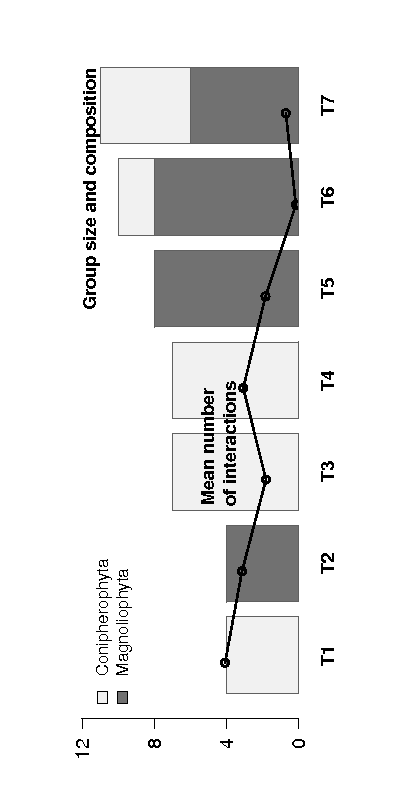
\includegraphics[height=.3\textwidth, width=.3\textwidth, trim=150 150 150 150]{\fignet/MRV10_AoAS_Q7_group}}
  \end{tabular}

}


%====================================================================
%====================================================================
\section{Extensions of block-models}
%====================================================================
\subsection{Covariates}
\frame{\frametitle{Outline} \tableofcontents[currentsection]}
%====================================================================
\frame{\frametitle{Accounting for covariates} 

  \paragraph{Adding a regression term.}
  \begin{itemize}
  \item Information about similarity or dissimilarity between species is often available \\
  \ra taxonomic, phylogenetic or geographic distance
  \item \bigskip Obvious generalization of the stochastic block-model \refer{MRV10}:
  $$
  Y_{ij} \sim \Pcal(\exp(\alpha_{Z_iZ_j} + x_{ij}^\intercal \beta))
  $$
  \ra $x_{ij} =$ vector of covariates for the pair $(i, j)$
  \item \bigskip Parameters: $\theta = (\pi, \alpha, \beta)$
  \end{itemize}

  \pause \bigskip \bigskip 
  \paragraph{Variational EM algorithm.} \refer{MRV10}
  \begin{itemize}
  \item Very similar to SBM without covariates
  \item \bigskip Estimation of $\beta$ via weighted generalized linear model
  \end{itemize}

}

%====================================================================
\frame{\frametitle{Tree species network} 

  \begin{tabular}{ccc}
    \hspace{-.04\textwidth}
    \begin{tabular}{p{.35\textwidth}}
      \paragraph{Covariate:}
      $$
      x_{ij} = \text{taxonomic distance}
      $$
      ~ \\

      \paragraph{Estimates:}
      $$
      \widehat{K}_{ICL} = 4
      $$
      $$
      \widehat{\beta} = -.317
      $$
      \onslide+<2->{\begin{itemize}
      \item Taxonomy (partially) explains the links (smaller $\widehat{K}$)
      \item \bigskip Distant species share less parasites ($\widehat{\beta} < 0$)
      \item \bigskip The remaining structure is \emphase{not related to taxonomy}
      \end{itemize}}
    \end{tabular}
    &
    \hspace{-.05\textwidth}
    \begin{tabular}{p{.3\textwidth}}
      \paragraph{No covariate:} $\widehat{K}_{ICL} = 7$ \\
      \includegraphics[height=.3\textwidth, width=.3\textwidth]{\fignet/Tree-adjMat-SBMnull} \\
      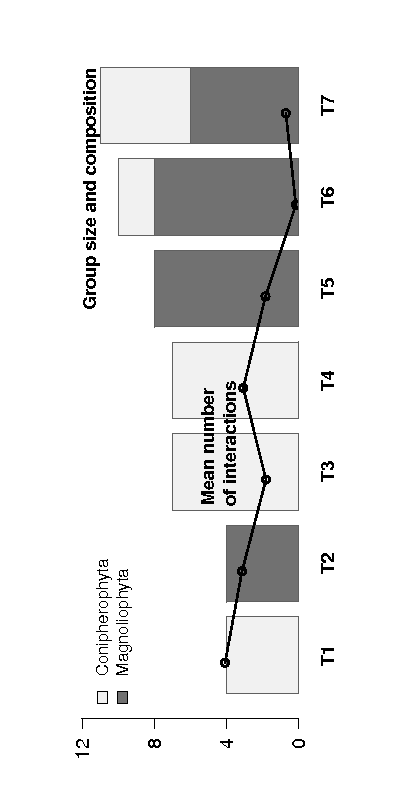
\includegraphics[height=.3\textwidth, width=.3\textwidth, trim=150 150 150 150]{\fignet/MRV10_AoAS_Q7_group}
    \end{tabular}
    &
    \hspace{-.05\textwidth}
    \begin{tabular}{p{.3\textwidth}}
      \paragraph{Taxonomic dist.:} $\widehat{K}_{ICL} = 4$ \\
      \includegraphics[height=.3\textwidth, width=.3\textwidth]{\fignet/Tree-adjMat-SBMtaxo} \\
      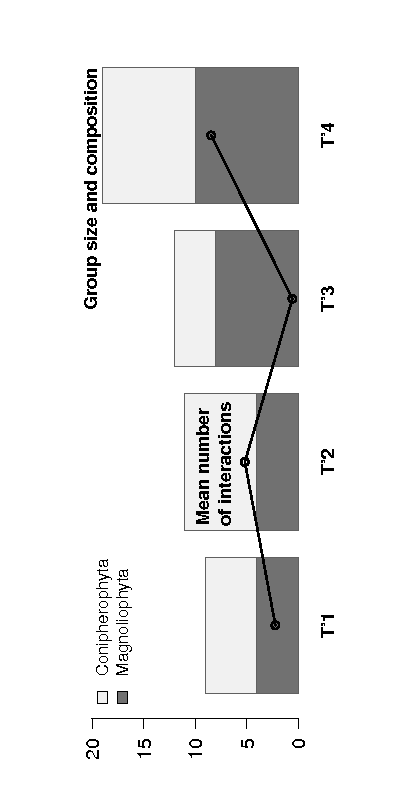
\includegraphics[height=.3\textwidth, width=.3\textwidth, trim=150 150 150 150]{\fignet/MRV10_AoAS_Q4_group}
    \end{tabular}
  \end{tabular}

}

%====================================================================
\subsection{Dynamic SBM}
%====================================================================
\frame{\frametitle{Animal behavior} 

  \paragraph{Data:} \refer{RSF15}
  \begin{itemize}
   \item Consider $n$ individuals (animals) along $T$ times (days, weeks)
   \item \bigskip At each time, observe
   $$
   Y_{ij}^t = \text{intensity of the social interaction between individuals $i$ and $j$ at time $t$}
   $$
  \end{itemize}
  
  \bigskip \bigskip \pause
  \paragraph{Questions:} 
  \begin{itemize}
  \item Do the individuals play different roles in the social network 
  \item \bigskip Do these roles change over time
  \end{itemize}

}

%====================================================================
\frame{\frametitle{Dynamic SBM} 

  \paragraph{Dynamic stochastic block-model.}   \refer{MaM17}
  \begin{itemize}
  \item Assume that individuals belong to $K$ clusters ('roles')
  \item \bigskip Denote by $Z_i^t$ the (latent) role of individual $i$ at time $t$
  \item \bigskip The successive roles of each individuals are independent Markov chains
  $$
  Z_i = \{Z_i^t\}_{1 \leq t \leq T} \sim MC(\nu_1, \pi)
  $$
  \item Social interactions are conditionally independent
  $$
  \{Y_{ij}^t\}_{i, j, t} \text{independent } \mid \{Z_i^t\}_{i, t}, \qquad
  Y_{ij}^t \mid Z_i^t, Z_j^t \sim F(\cdot; \gamma_{Z_i^t, Z_j^t})
  $$
  \end{itemize}  
  $$
  \begin{overprint}
    \onslide<2>  \begin{tikzpicture}
    \node[nocircle] (LL) at (-0.5*\edgeunit,-0.5*\edgeunit) {};
  \node[nocircle] (UL) at (-0.5*\edgeunit, 2.5*\edgeunit) {};
  \node[nocircle] (UR) at ( 5.0*\edgeunit, 2.5*\edgeunit) {};
  \node[nocircle] (UL) at ( 5.0*\edgeunit,-0.5*\edgeunit) {};

  \node[hidden] (Z11) at (0.0*\edgeunit,  2.0*\edgeunit) {$Z^1_1$};
  \node[hidden] (Z21) at (0.0*\edgeunit,  1.0*\edgeunit) {$Z^1_i$};
  \node[hidden] (Z31) at (0.0*\edgeunit,  0.0*\edgeunit) {$Z^1_n$};

  
\end{tikzpicture}

    \onslide<3>  \begin{tikzpicture}
    \node[nocircle] (LL) at (-0.5*\edgeunit,-0.5*\edgeunit) {};
  \node[nocircle] (UL) at (-0.5*\edgeunit, 2.5*\edgeunit) {};
  \node[nocircle] (UR) at ( 5.0*\edgeunit, 2.5*\edgeunit) {};
  \node[nocircle] (UL) at ( 5.0*\edgeunit,-0.5*\edgeunit) {};

  \node[hidden] (Z11) at (0.0*\edgeunit,  2.0*\edgeunit) {$Z^1_1$};
  \node[hidden] (Z21) at (0.0*\edgeunit,  1.0*\edgeunit) {$Z^1_i$};
  \node[hidden] (Z31) at (0.0*\edgeunit,  0.0*\edgeunit) {$Z^1_n$};

  \node[observed] (Y121) at (1.0*\edgeunit, 1.8*\edgeunit) {$Y^1_{1i}$};
  \node[observed] (Y131) at (1.0*\edgeunit, 1.0*\edgeunit) {$Y^1_{1n}$};
  \node[observed] (Y231) at (1.0*\edgeunit, 0.2*\edgeunit) {$Y^1_{in}$};
  

  
  \draw[arrow] (Z11) to (Y121);  \draw[arrow] (Z11) to (Y131);  
  \draw[arrow] (Z21) to (Y121);  \draw[arrow] (Z21) to (Y231);  
  \draw[arrow] (Z31) to (Y131);  \draw[arrow] (Z31) to (Y231);  
  
\end{tikzpicture}

    \onslide<4>  \begin{tikzpicture}
    \node[nocircle] (LL) at (-0.5*\edgeunit,-0.5*\edgeunit) {};
  \node[nocircle] (UL) at (-0.5*\edgeunit, 2.5*\edgeunit) {};
  \node[nocircle] (UR) at ( 5.0*\edgeunit, 2.5*\edgeunit) {};
  \node[nocircle] (UL) at ( 5.0*\edgeunit,-0.5*\edgeunit) {};

  \node[hidden] (Z11) at (0.0*\edgeunit,  2.0*\edgeunit) {$Z^1_1$};
  \node[hidden] (Z21) at (0.0*\edgeunit,  1.0*\edgeunit) {$Z^1_i$};
  \node[hidden] (Z31) at (0.0*\edgeunit,  0.0*\edgeunit) {$Z^1_n$};

  \node[hidden] (Z12) at (2.0*\edgeunit,  2.0*\edgeunit) {$Z^2_1$};
  \node[hidden] (Z22) at (2.0*\edgeunit,  1.0*\edgeunit) {$Z^2_i$};
  \node[hidden] (Z32) at (2.0*\edgeunit,  0.0*\edgeunit) {$Z^2_n$};

  \node[observed] (Y121) at (1.0*\edgeunit, 1.8*\edgeunit) {$Y^1_{1i}$};
  \node[observed] (Y131) at (1.0*\edgeunit, 1.0*\edgeunit) {$Y^1_{1n}$};
  \node[observed] (Y231) at (1.0*\edgeunit, 0.2*\edgeunit) {$Y^1_{in}$};
  

  
  \draw[arrow] (Z11) to (Y121);  \draw[arrow] (Z11) to (Y131);  
  \draw[arrow] (Z21) to (Y121);  \draw[arrow] (Z21) to (Y231);  
  \draw[arrow] (Z31) to (Y131);  \draw[arrow] (Z31) to (Y231);  
  
  \draw[arrowbendleft] (Z11) to (Z12);  
  \draw[arrowbendleft] (Z21) to (Z22);  
  \draw[arrowbendright] (Z31) to (Z32);
  
\end{tikzpicture}

    \onslide<5>  \begin{tikzpicture}
    \node[nocircle] (LL) at (-0.5*\edgeunit,-0.5*\edgeunit) {};
  \node[nocircle] (UL) at (-0.5*\edgeunit, 2.5*\edgeunit) {};
  \node[nocircle] (UR) at ( 5.0*\edgeunit, 2.5*\edgeunit) {};
  \node[nocircle] (UL) at ( 5.0*\edgeunit,-0.5*\edgeunit) {};

  \node[hidden] (Z11) at (0.0*\edgeunit,  2.0*\edgeunit) {$Z^1_1$};
  \node[hidden] (Z21) at (0.0*\edgeunit,  1.0*\edgeunit) {$Z^1_i$};
  \node[hidden] (Z31) at (0.0*\edgeunit,  0.0*\edgeunit) {$Z^1_n$};

  \node[hidden] (Z12) at (2.0*\edgeunit,  2.0*\edgeunit) {$Z^2_1$};
  \node[hidden] (Z22) at (2.0*\edgeunit,  1.0*\edgeunit) {$Z^2_i$};
  \node[hidden] (Z32) at (2.0*\edgeunit,  0.0*\edgeunit) {$Z^2_n$};

  \node[observed] (Y121) at (1.0*\edgeunit, 1.8*\edgeunit) {$Y^1_{1i}$};
  \node[observed] (Y131) at (1.0*\edgeunit, 1.0*\edgeunit) {$Y^1_{1n}$};
  \node[observed] (Y231) at (1.0*\edgeunit, 0.2*\edgeunit) {$Y^1_{in}$};

  \node[observed] (Y122) at (3.0*\edgeunit, 1.8*\edgeunit) {$Y^2_{1i}$};
  \node[observed] (Y132) at (3.0*\edgeunit, 1.0*\edgeunit) {$Y^2_{1n}$};
  \node[observed] (Y232) at (3.0*\edgeunit, 0.2*\edgeunit) {$Y^2_{in}$};
    

  
  \draw[arrow] (Z11) to (Y121);  \draw[arrow] (Z11) to (Y131);  
  \draw[arrow] (Z21) to (Y121);  \draw[arrow] (Z21) to (Y231);  
  \draw[arrow] (Z31) to (Y131);  \draw[arrow] (Z31) to (Y231);  
  
  \draw[arrowbendleft] (Z11) to (Z12);  
  \draw[arrowbendleft] (Z21) to (Z22);  
  \draw[arrowbendright] (Z31) to (Z32);
  
  \draw[arrow] (Z12) to (Y122);  \draw[arrow] (Z12) to (Y132);  
  \draw[arrow] (Z22) to (Y122);  \draw[arrow] (Z22) to (Y232);  
  \draw[arrow] (Z32) to (Y132);  \draw[arrow] (Z32) to (Y232);  

\end{tikzpicture}

    \onslide<6>  \begin{tikzpicture}
    \node[nocircle] (LL) at (-0.5*\edgeunit,-0.5*\edgeunit) {};
  \node[nocircle] (UL) at (-0.5*\edgeunit, 2.5*\edgeunit) {};
  \node[nocircle] (UR) at ( 5.0*\edgeunit, 2.5*\edgeunit) {};
  \node[nocircle] (UL) at ( 5.0*\edgeunit,-0.5*\edgeunit) {};

  \node[hidden] (Z11) at (0.0*\edgeunit,  2.0*\edgeunit) {$Z^1_1$};
  \node[hidden] (Z21) at (0.0*\edgeunit,  1.0*\edgeunit) {$Z^1_i$};
  \node[hidden] (Z31) at (0.0*\edgeunit,  0.0*\edgeunit) {$Z^1_n$};

  \node[hidden] (Z12) at (2.0*\edgeunit,  2.0*\edgeunit) {$Z^2_1$};
  \node[hidden] (Z22) at (2.0*\edgeunit,  1.0*\edgeunit) {$Z^2_i$};
  \node[hidden] (Z32) at (2.0*\edgeunit,  0.0*\edgeunit) {$Z^2_n$};

  \node[hidden] (Z13) at (4.0*\edgeunit,  2.0*\edgeunit) {$Z^3_1$};
  \node[hidden] (Z23) at (4.0*\edgeunit,  1.0*\edgeunit) {$Z^3_i$};
  \node[hidden] (Z33) at (4.0*\edgeunit,  0.0*\edgeunit) {$Z^3_n$};

  \node[nocircle] (Z14) at (6.0*\edgeunit,  2.0*\edgeunit) {};
  \node[nocircle] (Z24) at (6.0*\edgeunit,  1.0*\edgeunit) {};
  \node[nocircle] (Z34) at (6.0*\edgeunit,  0.0*\edgeunit) {};

  \node[observed] (Y121) at (1.0*\edgeunit, 1.8*\edgeunit) {$Y^1_{1i}$};
  \node[observed] (Y131) at (1.0*\edgeunit, 1.0*\edgeunit) {$Y^1_{1n}$};
  \node[observed] (Y231) at (1.0*\edgeunit, 0.2*\edgeunit) {$Y^1_{in}$};
  
  \node[observed] (Y122) at (3.0*\edgeunit, 1.8*\edgeunit) {$Y^2_{1i}$};
  \node[observed] (Y132) at (3.0*\edgeunit, 1.0*\edgeunit) {$Y^2_{1n}$};
  \node[observed] (Y232) at (3.0*\edgeunit, 0.2*\edgeunit) {$Y^2_{in}$};
  
  \node[observed] (Y123) at (5.0*\edgeunit, 1.8*\edgeunit) {$Y^3_{1i}$};
  \node[observed] (Y133) at (5.0*\edgeunit, 1.0*\edgeunit) {$Y^3_{1n}$};
  \node[observed] (Y233) at (5.0*\edgeunit, 0.2*\edgeunit) {$Y^3_{in}$};

  
  \draw[arrow] (Z11) to (Y121);  \draw[arrow] (Z11) to (Y131);  
  \draw[arrow] (Z21) to (Y121);  \draw[arrow] (Z21) to (Y231);  
  \draw[arrow] (Z31) to (Y131);  \draw[arrow] (Z31) to (Y231);  
  
  \draw[arrowbendleft] (Z11) to (Z12);  
  \draw[arrowbendleft] (Z21) to (Z22);  
  \draw[arrowbendright] (Z31) to (Z32);
  
  \draw[arrow] (Z12) to (Y122);  \draw[arrow] (Z12) to (Y132);  
  \draw[arrow] (Z22) to (Y122);  \draw[arrow] (Z22) to (Y232);  
  \draw[arrow] (Z32) to (Y132);  \draw[arrow] (Z32) to (Y232);  
  
  \draw[arrowbendleft] (Z12) to (Z13);  
  \draw[arrowbendleft] (Z22) to (Z23);  
  \draw[arrowbendright] (Z32) to (Z33);
  
  \draw[arrow] (Z13) to (Y123);  \draw[arrow] (Z13) to (Y133);  
  \draw[arrow] (Z23) to (Y123);  \draw[arrow] (Z23) to (Y233);  
  \draw[arrow] (Z33) to (Y133);  \draw[arrow] (Z33) to (Y233);  
  
  \draw[arrowbendleft] (Z13) to (Z14);  
  \draw[arrowbendleft] (Z23) to (Z24);  
  \draw[arrowbendright] (Z33) to (Z34);
  
\end{tikzpicture}

  \end{overprint}
  $$

}

%====================================================================
\frame{\frametitle{Variational EM} 

  \paragraph{Intractable EM.} Denoting $Z^t =(Z_1^t, \dots Z_n^t)$,  $(Z^t \mid Y)_{t \geq 1}$ is a Markov chain ... with $K^n$ states
  $$
  \begin{overprint}
   \onslide<2>  \begin{tikzpicture}
    \node[nocircle] (LL) at (-0.5*\edgeunit,-0.5*\edgeunit) {};
  \node[nocircle] (UL) at (-0.5*\edgeunit, 2.5*\edgeunit) {};
  \node[nocircle] (UR) at ( 5.0*\edgeunit, 2.5*\edgeunit) {};
  \node[nocircle] (UL) at ( 5.0*\edgeunit,-0.5*\edgeunit) {};

  \node[hidden] (Z11) at (0.0*\edgeunit,  2.0*\edgeunit) {$Z^1_1$};
  \node[hidden] (Z21) at (0.0*\edgeunit,  1.0*\edgeunit) {$Z^1_i$};
  \node[hidden] (Z31) at (0.0*\edgeunit,  0.0*\edgeunit) {$Z^1_n$};

  \node[hidden] (Z12) at (2.0*\edgeunit,  2.0*\edgeunit) {$Z^2_1$};
  \node[hidden] (Z22) at (2.0*\edgeunit,  1.0*\edgeunit) {$Z^2_i$};
  \node[hidden] (Z32) at (2.0*\edgeunit,  0.0*\edgeunit) {$Z^2_n$};

  \node[hidden] (Z13) at (4.0*\edgeunit,  2.0*\edgeunit) {$Z^3_1$};
  \node[hidden] (Z23) at (4.0*\edgeunit,  1.0*\edgeunit) {$Z^3_i$};
  \node[hidden] (Z33) at (4.0*\edgeunit,  0.0*\edgeunit) {$Z^3_n$};

  \node[nocircle] (Z14) at (6.0*\edgeunit,  2.0*\edgeunit) {};
  \node[nocircle] (Z24) at (6.0*\edgeunit,  1.0*\edgeunit) {};
  \node[nocircle] (Z34) at (6.0*\edgeunit,  0.0*\edgeunit) {};

  \node[observed] (Y121) at (1.0*\edgeunit, 1.8*\edgeunit) {$Y^1_{1i}$};
  \node[observed] (Y131) at (1.0*\edgeunit, 1.0*\edgeunit) {$Y^1_{1n}$};
  \node[observed] (Y231) at (1.0*\edgeunit, 0.2*\edgeunit) {$Y^1_{in}$};
  
  \node[observed] (Y122) at (3.0*\edgeunit, 1.8*\edgeunit) {$Y^2_{1i}$};
  \node[observed] (Y132) at (3.0*\edgeunit, 1.0*\edgeunit) {$Y^2_{1n}$};
  \node[observed] (Y232) at (3.0*\edgeunit, 0.2*\edgeunit) {$Y^2_{in}$};
  
  \node[observed] (Y123) at (5.0*\edgeunit, 1.8*\edgeunit) {$Y^3_{1i}$};
  \node[observed] (Y133) at (5.0*\edgeunit, 1.0*\edgeunit) {$Y^3_{1n}$};
  \node[observed] (Y233) at (5.0*\edgeunit, 0.2*\edgeunit) {$Y^3_{in}$};

  
  \draw[arrow] (Z11) to (Y121);  \draw[arrow] (Z11) to (Y131);  
  \draw[arrow] (Z21) to (Y121);  \draw[arrow] (Z21) to (Y231);  
  \draw[arrow] (Z31) to (Y131);  \draw[arrow] (Z31) to (Y231);  
  
  \draw[arrowbendleft] (Z11) to (Z12);  
  \draw[arrowbendleft] (Z21) to (Z22);  
  \draw[arrowbendright] (Z31) to (Z32);
  
  \draw[arrow] (Z12) to (Y122);  \draw[arrow] (Z12) to (Y132);  
  \draw[arrow] (Z22) to (Y122);  \draw[arrow] (Z22) to (Y232);  
  \draw[arrow] (Z32) to (Y132);  \draw[arrow] (Z32) to (Y232);  
  
  \draw[arrowbendleft] (Z12) to (Z13);  
  \draw[arrowbendleft] (Z22) to (Z23);  
  \draw[arrowbendright] (Z32) to (Z33);
  
  \draw[arrow] (Z13) to (Y123);  \draw[arrow] (Z13) to (Y133);  
  \draw[arrow] (Z23) to (Y123);  \draw[arrow] (Z23) to (Y233);  
  \draw[arrow] (Z33) to (Y133);  \draw[arrow] (Z33) to (Y233);  
  
  \draw[arrowbendleft] (Z13) to (Z14);  
  \draw[arrowbendleft] (Z23) to (Z24);  
  \draw[arrowbendright] (Z33) to (Z34);
  
\end{tikzpicture}

   \onslide<3>  \begin{tikzpicture}
    \node[nocircle] (LL) at (-0.5*\edgeunit,-0.5*\edgeunit) {};
  \node[nocircle] (UL) at (-0.5*\edgeunit, 2.5*\edgeunit) {};
  \node[nocircle] (UR) at ( 5.0*\edgeunit, 2.5*\edgeunit) {};
  \node[nocircle] (UL) at ( 5.0*\edgeunit,-0.5*\edgeunit) {};

  \node[hidden] (Z11) at (0.0*\edgeunit,  2.0*\edgeunit) {$Z^1_1$};
  \node[hidden] (Z21) at (0.0*\edgeunit,  1.0*\edgeunit) {$Z^1_i$};
  \node[hidden] (Z31) at (0.0*\edgeunit,  0.0*\edgeunit) {$Z^1_n$};

  \node[hidden] (Z12) at (2.0*\edgeunit,  2.0*\edgeunit) {$Z^2_1$};
  \node[hidden] (Z22) at (2.0*\edgeunit,  1.0*\edgeunit) {$Z^2_i$};
  \node[hidden] (Z32) at (2.0*\edgeunit,  0.0*\edgeunit) {$Z^2_n$};

  \node[hidden] (Z13) at (4.0*\edgeunit,  2.0*\edgeunit) {$Z^3_1$};
  \node[hidden] (Z23) at (4.0*\edgeunit,  1.0*\edgeunit) {$Z^3_i$};
  \node[hidden] (Z33) at (4.0*\edgeunit,  0.0*\edgeunit) {$Z^3_n$};

  \node[nocircle] (Z14) at (6.0*\edgeunit,  2.0*\edgeunit) {};
  \node[nocircle] (Z24) at (6.0*\edgeunit,  1.0*\edgeunit) {};
  \node[nocircle] (Z34) at (6.0*\edgeunit,  0.0*\edgeunit) {};

  \node[observed] (Y121) at (1.0*\edgeunit, 1.8*\edgeunit) {$Y^1_{1i}$};
  \node[observed] (Y131) at (1.0*\edgeunit, 1.0*\edgeunit) {$Y^1_{1n}$};
  \node[observed] (Y231) at (1.0*\edgeunit, 0.2*\edgeunit) {$Y^1_{in}$};
  
  \node[observed] (Y122) at (3.0*\edgeunit, 1.8*\edgeunit) {$Y^2_{1i}$};
  \node[observed] (Y132) at (3.0*\edgeunit, 1.0*\edgeunit) {$Y^2_{1n}$};
  \node[observed] (Y232) at (3.0*\edgeunit, 0.2*\edgeunit) {$Y^2_{in}$};
  
  \node[observed] (Y123) at (5.0*\edgeunit, 1.8*\edgeunit) {$Y^3_{1i}$};
  \node[observed] (Y133) at (5.0*\edgeunit, 1.0*\edgeunit) {$Y^3_{1n}$};
  \node[observed] (Y233) at (5.0*\edgeunit, 0.2*\edgeunit) {$Y^3_{in}$};
  

  % GG-dSBM
  \draw[arrow] (Z11) to (Y121);  \draw[arrow] (Z11) to (Y131);  
  \draw[arrow] (Z21) to (Y121);  \draw[arrow] (Z21) to (Y231);  
  \draw[arrow] (Z31) to (Y131);  \draw[arrow] (Z31) to (Y231);  
  
  \draw[arrowbendleft] (Z11) to (Z12);  
  \draw[arrowbendleft] (Z21) to (Z22);  
  \draw[arrowbendright] (Z31) to (Z32);
  
  \draw[arrow] (Z12) to (Y122);  \draw[arrow] (Z12) to (Y132);  
  \draw[arrow] (Z22) to (Y122);  \draw[arrow] (Z22) to (Y232);  
  \draw[arrow] (Z32) to (Y132);  \draw[arrow] (Z32) to (Y232);  
  
  \draw[arrowbendleft] (Z12) to (Z13);  
  \draw[arrowbendleft] (Z22) to (Z23);  
  \draw[arrowbendright] (Z32) to (Z33);
  
  \draw[arrow] (Z13) to (Y123);  \draw[arrow] (Z13) to (Y133);  
  \draw[arrow] (Z23) to (Y123);  \draw[arrow] (Z23) to (Y233);  
  \draw[arrow] (Z33) to (Y133);  \draw[arrow] (Z33) to (Y233);  
  
  \draw[arrowbendleft] (Z13) to (Z14);  
  \draw[arrowbendleft] (Z23) to (Z24);  
  \draw[arrowbendright] (Z33) to (Z34);
    
  \draw[lightedge] (Z11) to (Z21);  
  \draw[lightedgebendright] (Z11) to (Z31);  
  \draw[lightedge] (Z21) to (Z31);
  
  \draw[lightedge] (Z12) to (Z22);  
  \draw[lightedgebendright] (Z12) to (Z32);  
  \draw[lightedge] (Z22) to (Z32);
  
  \draw[lightedge] (Z13) to (Z23);  
  \draw[lightedgebendright] (Z13) to (Z33);  
  \draw[lightedge] (Z23) to (Z33);
  
\end{tikzpicture}

   \onslide<4->  \begin{tikzpicture}
    \node[nocircle] (LL) at (-0.5*\edgeunit,-0.5*\edgeunit) {};
  \node[nocircle] (UL) at (-0.5*\edgeunit, 2.5*\edgeunit) {};
  \node[nocircle] (UR) at ( 5.0*\edgeunit, 2.5*\edgeunit) {};
  \node[nocircle] (UL) at ( 5.0*\edgeunit,-0.5*\edgeunit) {};

  \node[hidden] (Z11) at (0.0*\edgeunit,  2.0*\edgeunit) {$Z^1_1$};
  \node[hidden] (Z21) at (0.0*\edgeunit,  1.0*\edgeunit) {$Z^1_i$};
  \node[hidden] (Z31) at (0.0*\edgeunit,  0.0*\edgeunit) {$Z^1_n$};

  \node[hidden] (Z12) at (2.0*\edgeunit,  2.0*\edgeunit) {$Z^2_1$};
  \node[hidden] (Z22) at (2.0*\edgeunit,  1.0*\edgeunit) {$Z^2_i$};
  \node[hidden] (Z32) at (2.0*\edgeunit,  0.0*\edgeunit) {$Z^2_n$};

  \node[hidden] (Z13) at (4.0*\edgeunit,  2.0*\edgeunit) {$Z^3_1$};
  \node[hidden] (Z23) at (4.0*\edgeunit,  1.0*\edgeunit) {$Z^3_i$};
  \node[hidden] (Z33) at (4.0*\edgeunit,  0.0*\edgeunit) {$Z^3_n$};

  \node[nocircle] (Z14) at (6.0*\edgeunit,  2.0*\edgeunit) {};
  \node[nocircle] (Z24) at (6.0*\edgeunit,  1.0*\edgeunit) {};
  \node[nocircle] (Z34) at (6.0*\edgeunit,  0.0*\edgeunit) {};

  \node[eliminated] (Y121) at (1.0*\edgeunit, 1.8*\edgeunit) {$Y^1_{1i}$};
  \node[eliminated] (Y131) at (1.0*\edgeunit, 1.0*\edgeunit) {$Y^1_{1n}$};
  \node[eliminated] (Y231) at (1.0*\edgeunit, 0.2*\edgeunit) {$Y^1_{in}$};
  
  \node[eliminated] (Y122) at (3.0*\edgeunit, 1.8*\edgeunit) {$Y^2_{1i}$};
  \node[eliminated] (Y132) at (3.0*\edgeunit, 1.0*\edgeunit) {$Y^2_{1n}$};
  \node[eliminated] (Y232) at (3.0*\edgeunit, 0.2*\edgeunit) {$Y^2_{in}$};
  
  \node[eliminated] (Y123) at (5.0*\edgeunit, 1.8*\edgeunit) {$Y^3_{1i}$};
  \node[eliminated] (Y133) at (5.0*\edgeunit, 1.0*\edgeunit) {$Y^3_{1n}$};
  \node[eliminated] (Y233) at (5.0*\edgeunit, 0.2*\edgeunit) {$Y^3_{in}$};
  

  % GG-dSBM
  \draw[lightedge] (Z11) to (Z12);  
  \draw[lightedge] (Z21) to (Z22);  
  \draw[lightedge] (Z31) to (Z32);
  
  \draw[lightedge] (Z12) to (Z13);  
  \draw[lightedge] (Z22) to (Z23);  
  \draw[lightedge] (Z32) to (Z33);
  
  \draw[lightedge] (Z13) to (Z14);  
  \draw[lightedge] (Z23) to (Z24);  
  \draw[lightedge] (Z33) to (Z34);
    
  \draw[lightedge] (Z11) to (Z21);  
  \draw[lightedgebendright] (Z11) to (Z31);  
  \draw[lightedge] (Z21) to (Z31);
  
  \draw[lightedge] (Z12) to (Z22);  
  \draw[lightedgebendright] (Z12) to (Z32);  
  \draw[lightedge] (Z22) to (Z32);
  
  \draw[lightedge] (Z13) to (Z23);  
  \draw[lightedgebendright] (Z13) to (Z33);  
  \draw[lightedge] (Z23) to (Z33);
  
\end{tikzpicture}

  \end{overprint}
  $$

  \onslide+<5->{\paragraph{Approximation classe.} $p_\theta(Z \mid Y) \simeq q(Z) =$ product of independent Markov chains (partial factorization) 
  $$
  \Qcal = \left\{q: 
  \quad q(Z) = \prod_i q_i(Z_i), 
  \quad q_i(Z_i) = q_i(Z_i^1) \prod_{t > 1} q_i(Z_i^t \mid Z_i^{t-1}) \right\}
  $$}
  
  \onslide+<6->{\paragraph{VEM algorithm.} 
  \begin{itemize}
    \item VE step = running $n$ forward-backward recursions
  \end{itemize}

  }

}

%====================================================================
\frame{\frametitle{Onager social network} 

  \paragraph{Data from \refer{RSF15}.} $n = 23$ onagers, observations gathered into $T=4$ time periods in \refer{MaM17}.
  $$
  \includegraphics[width=.5\textwidth]{\fignet/MaM17-JRSSB-Fig8b}
  $$
  
  \begin{itemize}
  \item \bigskip 4 groups (='roles') are found, from isolated to highly central
  \item \bigskip A fraction of individuals do change role from one period to another
  \end{itemize}

}

%====================================================================
\subsection{\textcolor{gray}{Metagenomics}}
%====================================================================
\frame{\frametitle{Latent block-model for comparative genomics} 

  \paragraph{Comparative metagnomics.}
  \begin{itemize}
  \item $n$ samples (soil surrounding the root of a plant --~{\sl rhizoshpere}~-- with given genotype), $p$ bacterial species ({\sl Operational Taxonomy Units} = OTUs), 
  \item \bigskip $Y_{ij} =$ number of reads from species $j$ in sample $i$
  \item \pause \bigskip \bigskip \emphase{Question:} Do preferential (or negative) associations exist between groups of genotypes and groups of bacteria?
  \item \bigskip \emphase{Over-dispersion:} Due to technological variability, counts are over-dispersed wrt Poisson \\
  \ra Negative-binomial (= Poisson-Gamma\footnote{$Y \sim \Ncal\text{eg}\Bcal\text{in}$
  \qquad $\Leftrightarrow$ \qquad $Y \sim \Pcal(\lambda U)$ \quad with $U \sim \Gcal\text{amma}$.
  }) distribution for the count
  \end{itemize}
}
  
%====================================================================
\frame{\frametitle{Latent block-model for comparative genomics} 

  \paragraph{Model.}
  \begin{itemize}
  \item \pause $\{Z_i\}_{1 \leq i \leq n}$ sample memberships (among $K$ groups) \textcolor{gray}{$\pi =$ proportions of sample groups}
  $$
  Z_i \sim \Mcal(1, \pi)
  $$
  \item \pause $\{W_j\}_{1 \leq j \leq p}$ species memberships (among $L$ groups) \textcolor{gray}{$\rho =$ proportions of species groups}
  $$
  W_i \sim \Mcal(1, \rho)
  $$
  \item \pause $\{U_{ij}\}_{1 \leq i \leq n, 1 \leq j \leq p}$ random effects \textcolor{gray}{$a =$ overdispersion parameter\footnote{The higher, the less dispersed.}}
  $$
  U_{ij} \sim \Gcal\text{amma}(a, a)
  $$
  \item \pause $\{Y_{ij}\}_{1 \leq i \leq n, 1 \leq j \leq p}$ observed counts \textcolor{gray}{$\mu_j =$ mean (log-)abundance of species $j$}
  $$
  Y_{ij} \sim \Pcal(\exp(o_i + \mu_j + \alpha_{\emphase{Z_iW_j}} + \emphase{\log U_{ij}}))
  $$
  $o_{ij} =$ known sampling effort for species $j$ in sample $i$
  \end{itemize}

  \pause \bigskip \bigskip 
  \paragraph{Parameters.}
  $$
  \theta = (\pi, \rho, a, \alpha, \mu) \qquad \qquad + (K, L)
  $$

}

%====================================================================
\frame{\frametitle{Rhizoshpere clustering} 

  \begin{tabular}{cc}
    \hspace{-.04\textwidth}
    \begin{tabular}{p{.55\textwidth}}
      \paragraph{Variational EM.} Using
      $$
      q(Z, W, U) = q_Z(Z) \; q_W(W) \; q_U(U)
      $$
      ~ \\ ~\\
      
      \paragraph{Model selection} with $vICL$ including $\Hcal(q_Z)$ and $\Hcal(q_W)$ \\
      ~ \\ ~\\ ~\\

      \pause \paragraph{Results.}
      \begin{itemize}
      \item $\widehat{K} = 4$ sample groups, $\widehat{L} = 10$ bacteria groups
      \item \bigskip Contrasted interactions: $\alpha_{kg} \in [-.5, 1.2]$
      \item \bigskip Sample groups display different biodiversity (Shannon index)
      \end{itemize}

    \end{tabular}
    &
    \begin{tabular}{p{.45\textwidth}}
      \includegraphics[width=.3\textwidth]{\figeco/ASR20-Preprint-Fig2right}\footnotetext[0]{$(Z, W)$ inverted in the figure}
    \end{tabular}
  \end{tabular}

}


% %====================================================================
%====================================================================
\section{Some more modeling problems}
\frame{\frametitle{Outline} \tableofcontents[currentsection]}
%====================================================================
\frame{\frametitle{Fundamental niche vs realized niche} 

}
  
%====================================================================
\frame{\frametitle{Noisy network inference} 

}
  



%====================================================================
%====================================================================
\section{To summarize}
\frame{\frametitle{Outline} \tableofcontents[currentsection]}
%====================================================================
\frame{\frametitle{To summarize} 

  \paragraph{VEM for latent models.}
  \begin{itemize}
   \item Latent variable models: flexible and explicit framework for modelling
   \item \bigskip Variational approximation: efficient approach for their inference \\
   \ra Mostly rely on the choice of the approximation class
  \end{itemize}

  \pause \bigskip \bigskip 
  \paragraph{Many other problems/models.}
  \begin{itemize}
   \item Account for a spatial structure, fundamental niche vs realized niche, looking for some structured in an inferred network, ...
  \end{itemize}

  \pause \bigskip \bigskip 
  \paragraph{Statistical guarantees.}
  \begin{itemize}
   \item General properties of variational estimates?
   \item \bigskip Combining VEM with other inference methods
  \end{itemize}


}
  


%====================================================================
%====================================================================
\backupbegin 
\section*{Backup}
%====================================================================
\frame[allowframebreaks]{ \frametitle{References}
  {\tiny
   \bibliography{/home/robin/Biblio/BibGene}
   \bibliographystyle{alpha}
  }
}

%====================================================================
%====================================================================
\section*{Backup}
%====================================================================



%====================================================================
\backupend 

%====================================================================
%====================================================================
\end{document}
%====================================================================
%====================================================================

  \begin{tabular}{cc}
    \hspace{-.04\textwidth}
    \begin{tabular}{p{.5\textwidth}}
    \end{tabular}
    &
    \begin{tabular}{p{.45\textwidth}}
    \end{tabular}
  \end{tabular}

